
\begin{figure}

\caption{Data Microcitations via Tabular Columns}
\label{fig:oxy}

\begin{tikzpicture}

\node[inner sep=0pt] (x1) at (0,0)
    {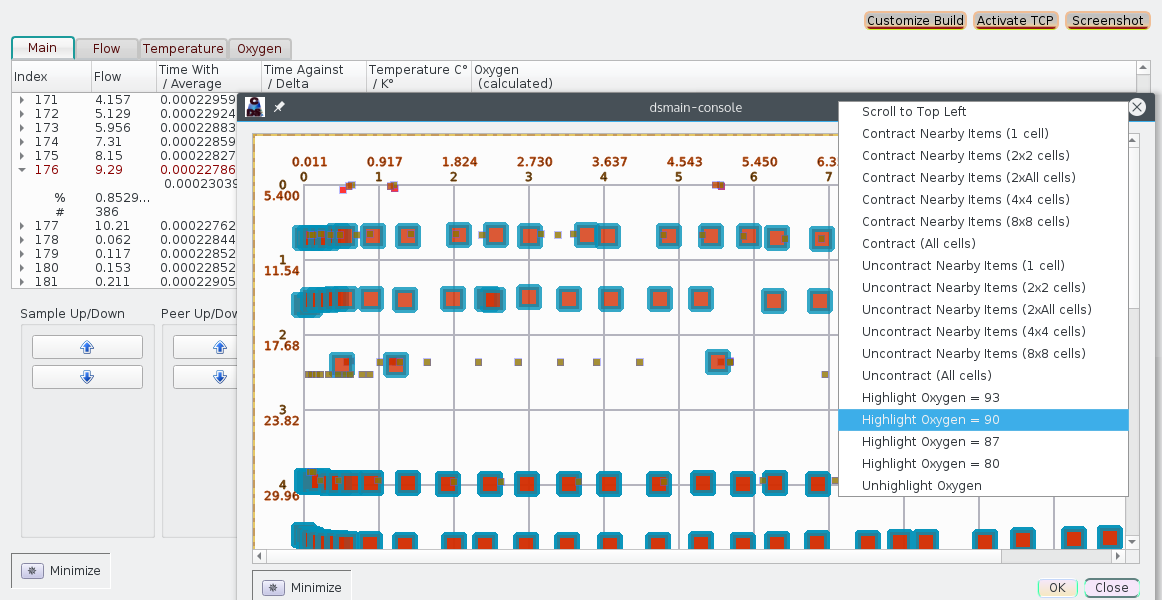
\includegraphics[width=180mm, 
    	trim={0mm 0mm 0mm 0mm},clip]
    	{pics/oxy.png}};
    
\end{tikzpicture}   
\end{figure}


\p{As outlined above, data citations refer to parts within a 
data set --- such as individual data records, but also larger-scale 
aggregates such as table columns or statistical parameters.  
The complication when defining data citations is that a 
concept such as a table column, although it may have an 
obvious technical status as a discrete conceptual unit from 
the point of view of scientists curating, studying or reusing 
a data set, does not necessarily correspond to a single 
coding entity that could be isolated as an annotation 
target.  It is therefore the responsibility of 
\textit{code base annotations} to provide annotations for 
computational units --- such as data types, procedures, and 
\GUI{} components --- that have an annotatable \textit{conceptual} 
status relative to the data set on which the code operates.  
Often this will involve mapping one concept to 
several computational units (for instance, several 
procedure implementations).}

\p{For a concrete example of these points concerning 
data citations, consider the data set pictured 
in Figure~\bref{fig:oxy}, representing cyber-physical measurements 
used to calculate oxygenated airflow.  The data-set 
application (interactive-visualization code deployed within 
the Research Object) displays tabular data via a tree widget 
(which functions as a generalized, multi-scale spreadsheet 
table), with tabular columns expressing quantities --- such 
as air flow and oxygen levels --- in several formats (raw 
measures as well as sample rankings and min-max 
percentages).  Conceptually, these columns have distinct 
methodological roles and therefore can be microcited; 
indeed, the application links the columns to article 
text where the corresponding concepts are presented 
(see Figure~\bref{fig:about}).  However, the implementation does not introduce 
a distinct \Cpp{} object uniquely designating individual 
columns.  Instead, the individual columns can be annotated 
in terms of \Cpp{} methods providing column-specific 
functionality.  In the current example, these methods 
primarily take the form of features linked to context-menu 
actions (copying column data to the clipboard, sorting data 
by one column, etc.).  In general, rather than a rigid 
protocol for data-set annotations, \AXF{} proposes 
heuristic guidelines for how best to map programming 
constructs to scientifically salient data-set concepts.}


\begin{figure}

\caption{Linking Dataset Applications to Publications}
\label{fig:about}

\begin{tikzpicture}

\node[inner sep=0pt] (x1) at (0,0)
    {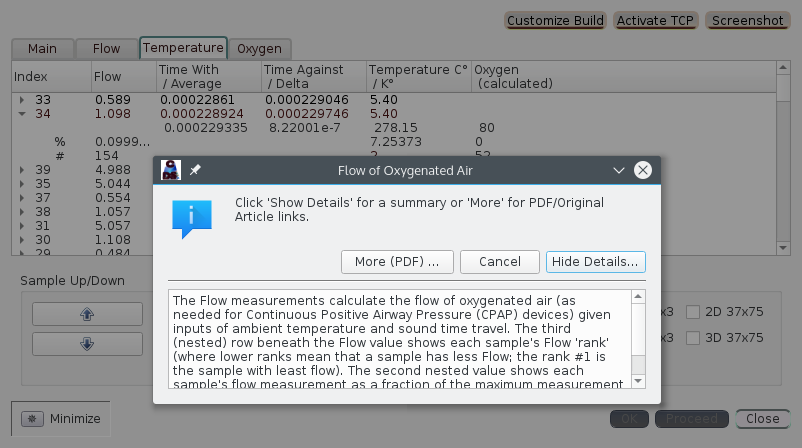
\includegraphics[width=180mm, 
    	trim={0mm 0mm 0mm 0mm},clip]
    	{pics/about.png}};

\end{tikzpicture}    
\end{figure}


\p{Defining an annotation schema for data sets can potentially 
be an organic outgrowth of software-development methodology 
--- viz., the engineering steps, 
such as implementing unit tests, which are essential 
to deploying a commercial-grade application.  
This point is illustrated in 
Figure~\bref{fig:testing}, which shows a \GUI{}-based testing environment for 
the data set depicted in Figures~\bref{fig:oxy} and 
\bref{fig:about}.  For this data set, 
the context menu actions providing column-specific functionality 
are also discrete capabilities which can be covered by 
unit tests, so the set of procedures mapped to the citeable 
concept correspond with a set of unit-test requirements.  
In this data set, these procedures are also exposed to 
scripting engines via the \Qt{} meta-object system.  In general, 
there is often a structural correlation between 
scripting, unit testing, and microcitation, so that 
an applications' scripting and testing protocol can serve 
as the basis for annotation schema.  For data sets which use 
in-memory or persistent databases, evaluable queries against 
these databases provide an additional grounding for annotations.  
In general, data-annotation should be engineered on the 
basis of a dataset applications' scripting, testing, and/or 
query-evaluation code.  However, this is only a heuristic 
guideline, and \AXF{} does not presuppose any data-annotation 
scheme \textit{a priori}.}

    \begin{frame}{\ft{Testing}}

        \begin{annotatedFigure}{0pt}{0pt}
            {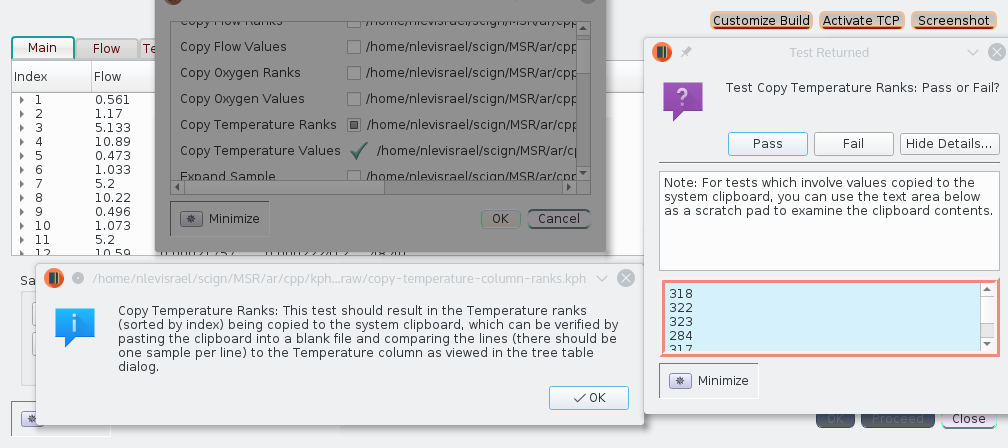
\includegraphics[scale=1]{texs/testing.png}}
            
  \node [text width=20cm,align=justify,fill=logoCyan!20, draw=logoBlue, 
  draw opacity=0.5,line width=1mm, fill opacity=0.9]
   at (0.38,0.93){\textbf{Dataset Creator includes a sophisticated 
   framework for building and running test suites to 
   ensure that raw data is processed correctly and that 
   User Interface components work properly on different 
   Operating System platforms.  This includes 
   a separate testing application that sends instructions 
   to the main Dataset Application via TCP (\circled{1}).}};

  \annotatedFigureBox{0.81,0.93}{0.903,0.982}{1}{0.903,0.935}%
  
  
   \node [text width=4cm,align=justify,fill=logoCyan!20, draw=logoBlue, 
   draw opacity=0.5,line width=1mm, fill opacity=0.9]
    at (0.08,0.64){\textbf{The testing application has several 
    features to facilitate running tests, including 
    options to repeat tests, mark success or failure (\circled{2}), and 
    examine the system clipboard (\circled{3}).}};
 
  \annotatedFigureBox{0.17,0.63}{0.37,0.685}{2}{0.37,0.63}
   \annotatedFigureBox{0.651,0.113}{0.995,0.86}{3}{0.892,0.86}% 

   \node [text width=11cm,align=justify,fill=logoCyan!20, draw=logoBlue, 
   draw opacity=0.5,line width=1mm, fill opacity=0.9]
    at (0.26,0.09){\textbf{Testers can 
    also read a description of each test (\circled{4}),  
    and view the scripts used to ceate them.}};
 
  \annotatedFigureBox{0.05,0.16}{0.62,0.325}{4}{0.62,0.19}
  
      %      \annotatedFigureBox{0.222,0.284}{0.3743,0.4934}{B}{0.3743,0.4934}%tr
      %      \annotatedFigureBox{0.555,0.784}{0.6815,0.874}{C}{0.555,0.784}%bl
      %      \annotatedFigureBox{0.557,0.322}{0.8985,0.5269}{D}{0.8985,0.5269}%tr
  
        \end{annotatedFigure}

    \end{frame}




